%! TEX root = ../main.tex
% =============================================================
% IMMUTABLE — generated automatically, do not edit this block
%   script          : analysis_scratch/reconstruction_A_vs_B.py
%   plot_type       : reconstruction_AvsB
%   chapter         : 04
%   demo_run        : 1.4 Hz, 0.2 V, full panel
%   band_half_hz    : 0.05
%   wind_band_hz    : 2.0-6.0
%   probes          : 9373/170, 12400/250
%   n_thesis_scope  : 156
%   ewind_absmax    : 0.0000%%
%   bandpeak_max    : 1.000000
%   findings_doc    : analysis_scratch/reconstruction_A_vs_B_findings.md
% =============================================================
\begin{figure}[htbp]
  \centering
  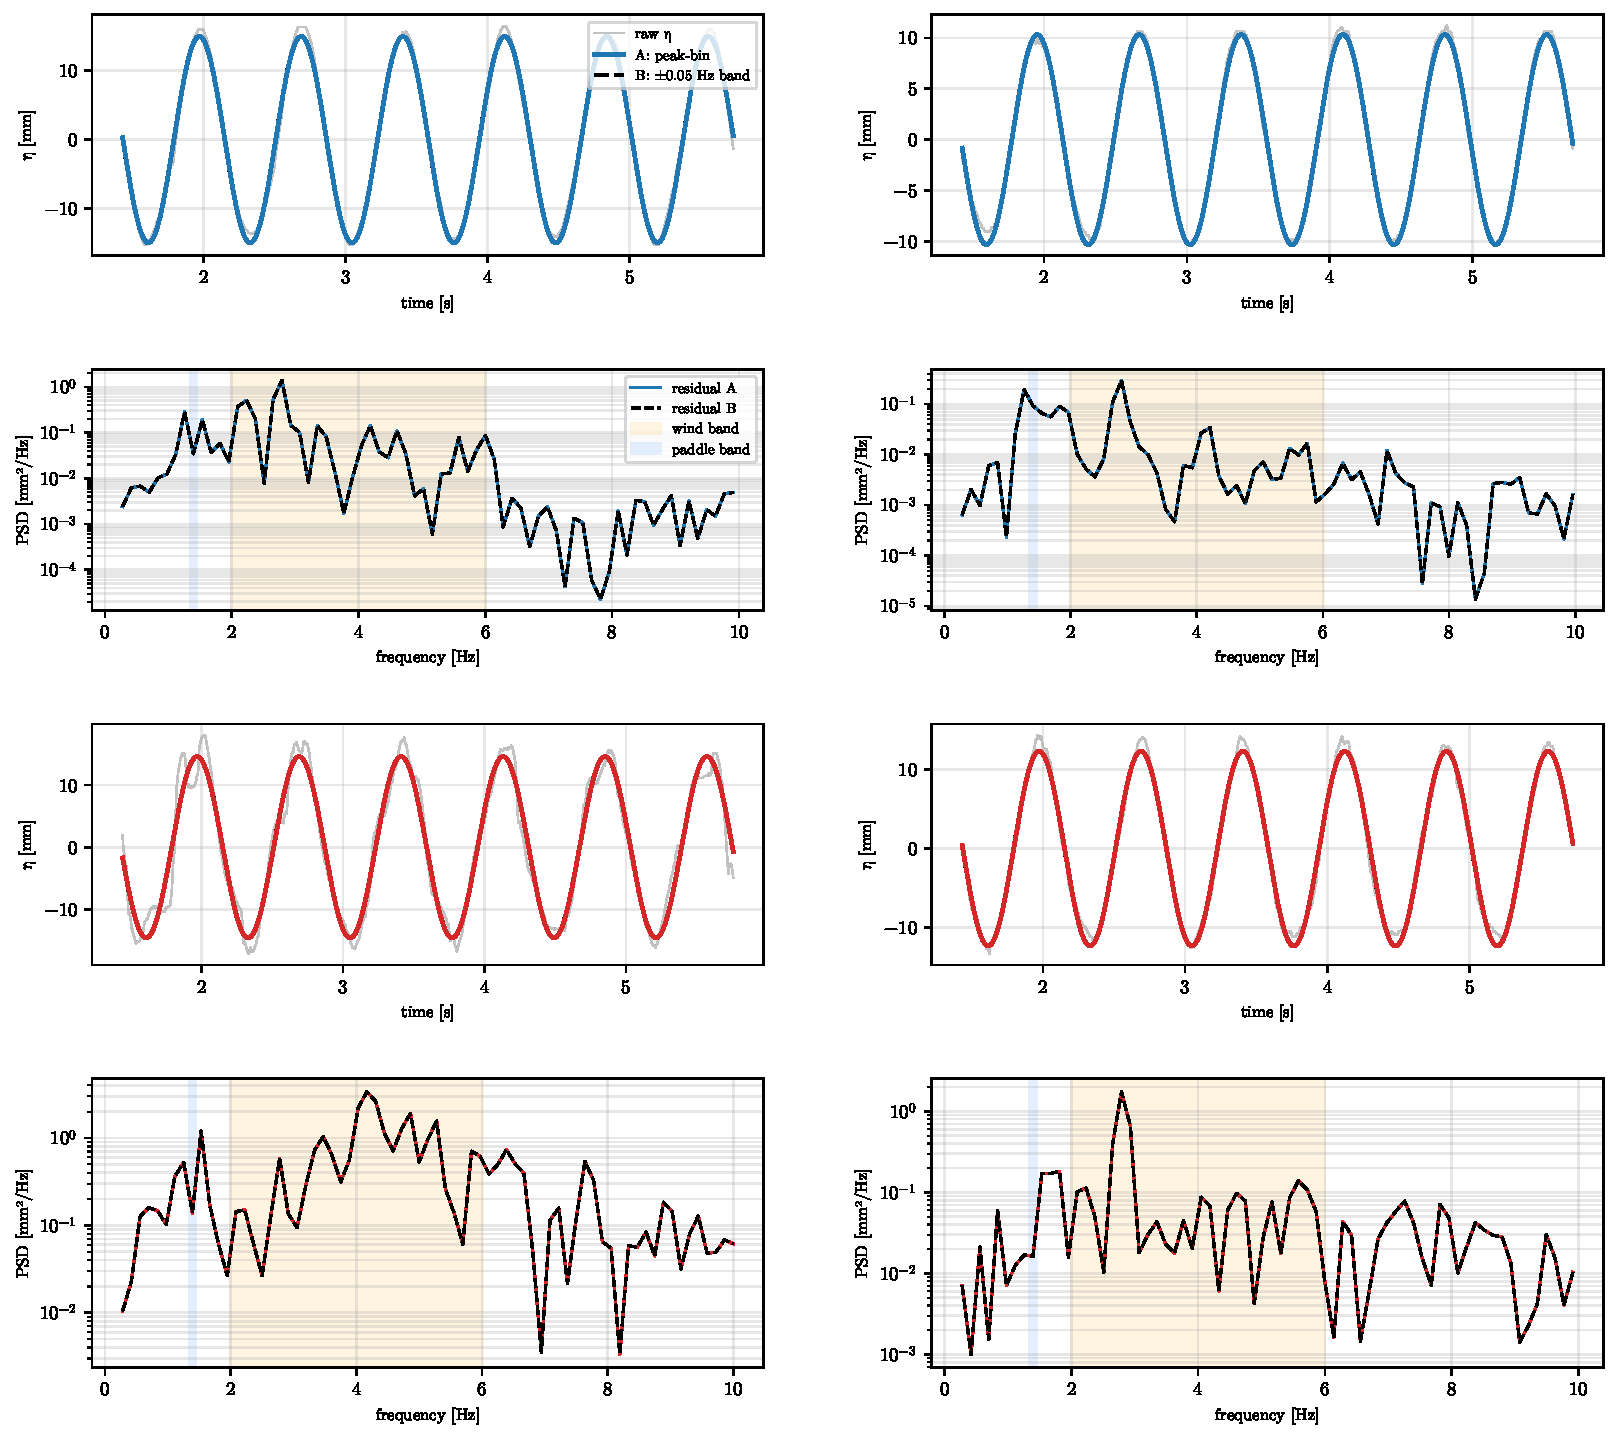
\includegraphics[width=0.98\linewidth]{FIGURES/ch04_reconstruction_AvsB.pdf}
  \caption[Peak-bin vs band-integrated reconstruction equivalence]{%
    Peak-bin (method A, solid blue) and band-integrated (method B, dashed red) reconstructions of the paddle wave at the IN probe (left) and OUT probe (right) under no-wind (rows 1--2) and full-wind (rows 3--4) conditions at the representative run $f=1.4$\,Hz, $A=0.20$\,V, full panel. Odd rows overlay the two reconstructions on the raw signal; even rows show the corresponding residual power spectra (log scale). Shaded bands mark the paddle band ($\pm 0.05$\,Hz around the paddle peak, blue) and the wind band (2--6\,Hz, orange). Across all thesis-scope runs ($f \in [1.3,1.6]$\,Hz, $n=156$ probe$\times$run pairs) the two reconstructions give identical wind-band residual energy to four-decimal precision and amplitude ratio $A_\mathrm{B}/A_\mathrm{A}=1.0000$. Any wind characterisation based on the method-A residual is therefore equivalent to one based on method B: the paddle-band sinc-leakage that A misses stays pinned inside the paddle band and does not contaminate the wind band.
  }
  \label{fig:ch04_reconstruction_AvsB}
\end{figure}
